% !TeX root = ../../thesis.tex
\chapter{Applications: Mandible plate}\label{ch:mandible}

\begin{shaded}
This chapter is based on submitted content to the \textit{Journal of the Mechanical Behavior of Biomedical Materials}:\\
P. Ansoms, M. Barzegari, and L. Geris, ``Coupling biomechanical models of implants with biodegradation models: a case study for biodegradable mandibular bone fixation plates,'' submitted to \textit{Journal of the Mechanical Behavior of Biomedical Materials}, 2022.
\end{shaded}

\section{Introduction}

In bone tissue engineering, biodegradable implants have gained in popularity over recent years. The main advantage of biodegradable implants over non-biodegradable implants is that no second surgery is needed to remove the implant after successful healing of the bone \cite{Zheng2014}. The removal of a non-biodegradable implant might be necessary to avoid complications in the long term and brings along an additional cost and risk of infection. Two other side effects of permanent implants are late thrombosis and chronic inflammation \cite{KChen}. Late thrombosis is the formation of blood cloths due to the presence of the metallic implant \cite{thrombosis}. Chronic inflammation is induced by the persistence of inflammatory stimuli, being the physical presence of the implanted biomaterial or the ability of the implant to slightly move at the implant site \cite{inflammation}. Permanent metallic implants also distort diagnostic images of the body \cite{Han}. Both in the short and long term, a biodegradable implant reduces stress shielding, which is the reduction in bone density as a result of removal of stress on the bone. The reduction of stress shielding in the long term is obvious since the the implant has disappeared in case of a biodegradable implant. The reduction of stress shielding in the short term results from the fact that biodegradable metals often have a Young's modulus that is much lower than that of inert metals (e.g. 44 GPa for WE43 vs. 118 GPa for Ti6Al4V). The stress shielding effect is directly proportional to the E-modulus of the implant material.

The use of biodegradable metals to support tissue regeneration is mentioned in various sources, describing different applications \cite{KChen,JChen,Yang}. The material of the implant determines the rate of degradation. The goal is to provide stable mechanical support at the early stage of the tissue healing process and then have the material gradually degrade with the restoration of the defect tissue \cite{Yang}. Fig. \ref{fig:rateofdeg} qualitatively shows the degradation rate of three common biomaterials (magnesium, zinc, and iron) along with the healing rate of different tissues (hard, soft and vascular) as an illustration. By matching a material's degradation rate and a tissue's healing rate, a suiting material can be found for a certain application.

\begin{figure}[ht]
    \centering
    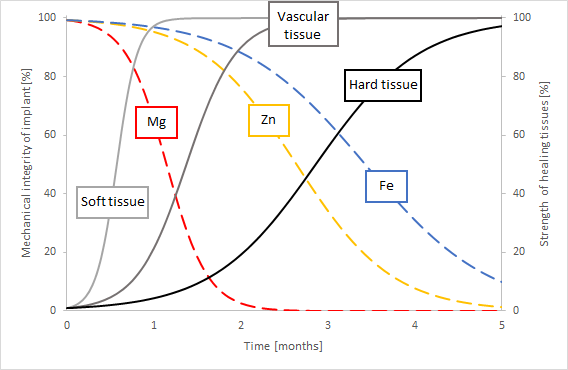
\includegraphics[width=0.86\textwidth]{MechanicalIntegrityTissueStrength.png}
    \caption{The change in mechanical integrity of the implant and tissue strength over time (Adapted from Chen et al. \cite{KChen})}
    \label{fig:rateofdeg}
\end{figure}

Studying the change of mechanical support of implants due to biodegradation has certain complexities. This case-study aimed to gain insight into the change in mechanical behavior of a biodegradable mandibular fixation plate. In order to do this, three different models should be combined: a biodegradation model to characterize the geometry change as a result of biodegradation, a model to characterize the loading on the jaw plate by considering the bone healing, and a model to predict the mechanical behavior of the plate. 

% very short discussion on mandible fractures
The mandible is the second most frequently fractured bone of the face and the tenth most frequently fractured bone of the body \cite{Bhavik}. Common causes for a mandible fracture are violence, car crashes and sports. It occurs more frequently for males than for females and most often between the ages of 16 and 30. The weakest section of the mandible is the angle because there is an abrupt change in direction between the body and ascending ramus, both in the sagittal and transverse planes, resulting in the involvement of the mandibular angle in jaw fractures in up to 28.5\% of cases \cite{Levy}. The treatment of mandible fractures is most commonly done with a mandibular fixation plate (further referred to as jaw plate) to stabilize the fracture and allow the healing process to take place. The plate is traditionally made of an inert implant material (e.g. titanium), which implies that it has minimal interaction with the surrounding tissues. Alternatively, the implant can be made from biodegradable materials to take advantage of the aforementioned benefits. 

The outcome of different surgeries on the mandible has been modelled by several studies \cite{Vautrin2021}. Zheng et al. were able to evaluate the impact of mandibular reconstruction surgery on the muscular functionality by developing a static FE model \cite{Zheng2019}. A topology optimization was performed by Wu et al. for a similar application, with the inclusion of a bone remodeling algorithm \cite{Wu2020}. Boccaccio et al. studied distraction osteogenesis of the mandible with a focus on tissue differentiation \cite{Boccaccio2008}. These models incorporated the tissue regeneration, but did not incorporate a biodegradable fixation system. The combination of concurrent biodegradation and bone regeneration has been developed for long bones by Mehboob et al. \cite{Mehboob2015} and by Ma et al. \cite{Ma2018}. Vautrin et al. even developed a combined biodegradation and tissue regeneration model in the context of orthognatic surgery \cite{Vautrin2021}. The bone healing algorithm was based on the model that Alierta et al. developed, but was generalized to be applicable to a larger fracture gap \cite{Alierta2013}. It modeled the growth of the contribution of cartilage and bone to the mechanical properties of each element within the fracture gap based on the principal element strains under physiological loading. The biodegradation algorithm was limited to being phenomenological to reduce the computational cost. It included only localized corrosion by incorporating a random pitting corrosion algorithm. 

The present work incorporated a more detailed biodegradation algorithm based on the chemistry of biodegradation of WE43. The tissue regeneration algorithm, on the other hand, made use of beam theory which was made possible by the specific type of fixation that was considered. The case-study focuses on investigating the effect of the number of plate holes left unscrewed and the impact of biodegradation on mechanical support in this condition.


\section{Materials and methods}

\subsection{Case study}

The implant for this case study was a jaw plate based on the one shown in Fig. \ref{fig:JPAO}. This technique of mandibular fracture fixation is called the 'miniplate fixation technique', also known as 'semi-rigid' or 'functionally adequate fixation'. The loading on the plate in this situation is purely tensile when a mastication load is applied. This is shown in Fig. \ref{fig:anteriorforce}. Fig. \ref{fig:BPpart} shows the plate that was used for this case study, and Fig. \ref{fig:JPscrews} shows the use of different amounts of screws for fixation. This was implemented to investigate the effect of leaving holes open and exposed to body fluids. Leaving holes open is a common thing because in some cases the location of a screw may be too close to a fracture line or in a section of the bone that is simply too weak. The details about the geometry are given in section \ref{sec:FEA}. Leaving a hole open is reflected both in the boundary conditions and in the degradation behavior of the simulation since it is assumed that a screw closes a hole off from body fluids and hence prohibits degradation within the screw hole.

%miniplate fixation
\begin{figure}[h]
    \centering
    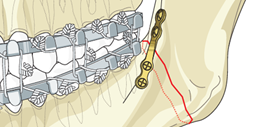
\includegraphics[width=0.6\textwidth]{JPAO.png}
    \caption{Miniplate fixation by AO Surgery Foundation \cite{JPAO}}
    \label{fig:JPAO}
\end{figure}

%occurrence of tensile and compressive forces
\begin{figure}[h]
    \centering
    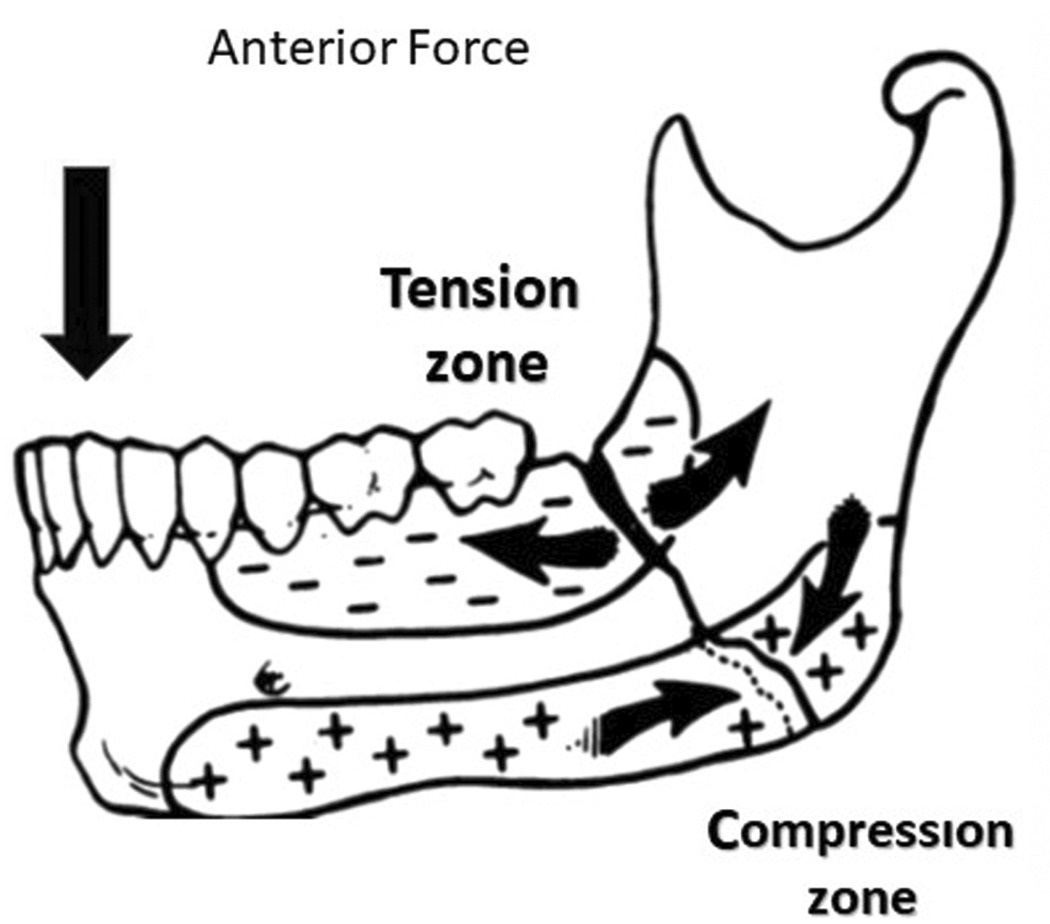
\includegraphics[width=0.57\textwidth]{anteriorforce.jpg}
    \caption{Occurrence of compressive- and tensile stresses around the fracture site when biting \cite{Bohluli}}
    \label{fig:anteriorforce}
\end{figure}

%geometry
\begin{figure}[h]
    \centering
    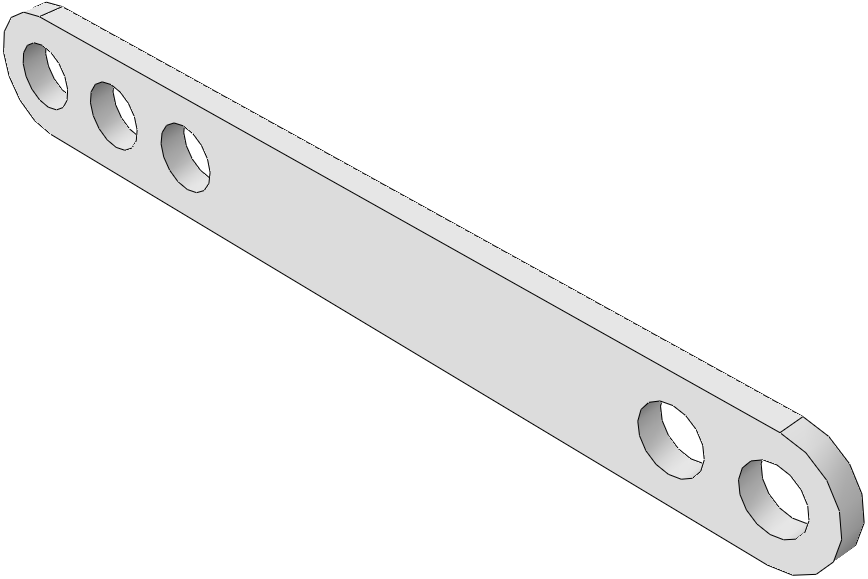
\includegraphics[width=0.7\textwidth]{BPpartcomp(5screws).png}
    \caption{Model for the jaw plate}
    \label{fig:BPpart}
\end{figure}

%different amount of screws
\begin{figure}[h]
  \centering
  \begin{minipage}[b]{0.51\textwidth}
    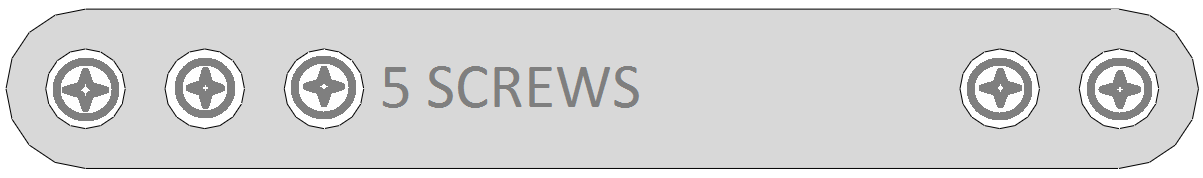
\includegraphics[width=\textwidth]{JParticle5.png}
    \captionsetup{labelformat=empty}
  \end{minipage}
  \hfill
  \begin{minipage}[b]{0.51\textwidth}
    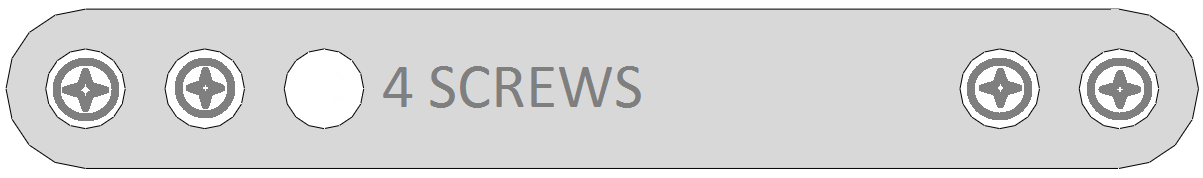
\includegraphics[width=\textwidth]{JParticle4.png}
    \captionsetup{labelformat=empty}
  \end{minipage}
  \hfill
  \begin{minipage}[b]{0.51\textwidth}
    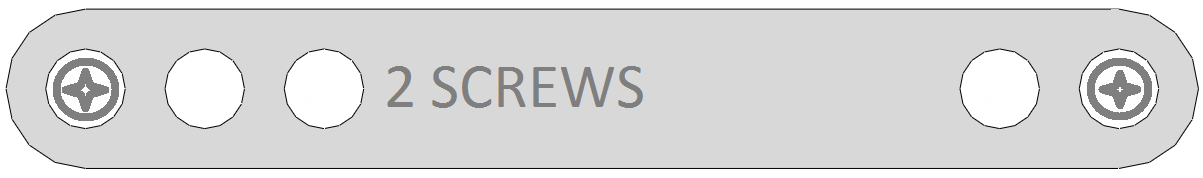
\includegraphics[width=\textwidth]{JParticle2.png}
    \captionsetup{labelformat=empty}
  \end{minipage}
  \caption{Five, four or two screws}
  \label{fig:JPscrews}
\end{figure}


\subsection{Biodegradation behavior simulation}

In the current study, the degradation was considered in simulated body fluids (SBF) solutions, which are the most similar buffered solutions to the body environment and are designed to mimic the surrounding environment of implants and medical devices \textit{in vitro}. The biodegradation process was modeled as a set of partial differential equations (PDEs), formulating the mass transfer phenomena as well as tracking the location of the surface of the implant during degradation. For the mass transfer model, a system of time-dependent reaction-diffusion PDEs was derived from the underlying oxidation-reduction reactions in SBF solutions. This includes the oxidation of the metallic part, reduction of water and oxygen, changes in pH, the effect of different ions in the medium, and formation of a protective film on the surface of the scaffold, slowing down the rate of degradation. Additionally, investigating the structural changes of implants requires monitoring the morphological changes, which was achieved by tracking the movement of the corrosion front. This was done by constructing an equation based on the Level Set formalism, capturing the movement of the environment-implant interface by defining an implicit surface. So, the zero-iso contour of this implicit Level set function determines the surface of the implant. The derived equations were coupled and solved implicitly using the finite element method, implemented in FreeFEM \cite{Hecht2012}. Experimental data to validate the developed biodegradation model were collected from immersion tests of simple blocks. More details of the model implementation and validation can be found in our previous work \cite{Barzegari2021}. Moreover, the mesh was refined adaptively on the corrosion front to increase the numerical accuracy of the interface tracking equation, leading to a computational-intensive model. So, in order to increase performance and reduce the simulation time, the code was parallelized in a way that the computation could be distributed across several computing nodes. This was mainly achieved using domain decomposition techniques and high-performance solvers. More information about this efficient implementation as well as a performance analysis of the model is presented in our previous work \cite{Barzegari2022}.

For the biodegradation simulation, the jaw plate was embedded into a cubic container acting as the surrounding environment. As mentioned above, the mesh was refined on the metal bulk interface, leading to a mesh comprising of $\num{19924153}$ elements and $\num{3316135}$ degrees of freedom (DOF) for each PDE. The material properties, including the diffusion coefficient of various contributing ions and reaction rates were set to mimic the degradation condition in SBF. The preferred values for SBF solutions as well the process for obtaining them is described in detail in our previous contribution \cite{Barzegari2021}. The biodegradation simulation was carried out using 170 computing cores.

\subsection{Mechanical behavior simulations}
\label{sec:FEA}

The finite element (FE) method was used to characterize the mechanical behavior of the degrading jaw plate. The simulations reflected tensile tests with different amounts of degradation, corresponding to a different point in time during the biodegradation process. Force-displacement curves were recorded during the analysis, from which the maximum bearable force was extracted to characterize the mechanical behavior. The analyses were performed in Abaqus/CAE v6.11 (Dassault Systèmes, USA). The type of analysis was explicit/dynamic. The explicit/dynamic analysis is a technique for the integration of the equations of motion through time. It calculates the next state of the system based on the previous state and in this way calculates motion iteratively. As a result, the system is not unconditionally stable, in contrast to a standard analysis. Therefore, sufficiently small time steps are required to ensure a stable calculation. Explicit dynamic analyses are useful in problems with high-speed dynamics, but also in quasi-static problems with large non-linear deformations and in highly discontinuous post-buckling and collapse simulations \cite{explicit2}. So, this is an ideal type of analysis for the simulation of tensile tests, in which failure of the material occurs. The simulations were performed on a machine with a 32-core AMD EPYC 7551 processor @2.00GHz and 64GB of RAM.

The material model for the simulations was based on WE43, which is a magnesium alloy with yttrium, zirconium, and rare earth elements added. Table \ref{tab:WE43} lists the properties that are important for the simulations. The true stress-strain relationship in the plastic region had to be specified for the plastic deformation behavior, so a stress-strain curve of WE43 from literature was used, shown in Fig. \ref{fig:WE43}.

\begin{table}[h]
\centering
\begin{tabular}{|l|l|l|} 
\hline
\textbf{Parameter} & \textbf{Value} & \textbf{Units}  \\ 
\hline
Density            & 1800           & kg/m$^3$        \\ 
\hline
E-modulus          & 44.2E+09       & Pa              \\ 
\hline
Poisson's ratio    & 0.27           & -               \\ 
\hline
Fracture strain    & 0.04           & -               \\ 
\hline
Yield stress       & 1.6E+08        & Pa              \\
\hline
\end{tabular}
\caption{Material parameters for WE43}
\label{tab:WE43}
\end{table}

\begin{figure}
\begin{minipage}[t]{0.59\textwidth}
%\begin{figure}[h]
    \centering
    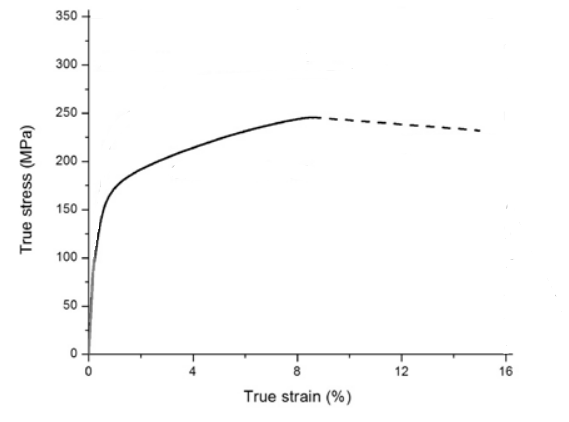
\includegraphics[width=\textwidth]{WE43.PNG}
%\end{figure}
\end{minipage}
\begin{minipage}[t]{0.4\textwidth}
%\begin{table}[h]
%\centering
\vspace{-50mm}
\begin{tabular}{|l|l|}
\hline
\textbf{True stress} & \textbf{True strain} \\
\multicolumn{1}{|c|}{{[}Pa{]}} & \multicolumn{1}{c|}{{[}-{]}} \\\hline
1.6E+08                       & 0                            \\ \hline
1.62E+08                      & 0.002                        \\ \hline
1.75E+08                      & 0.01                         \\ \hline
1.88E+08                      & 0.02                         \\ \hline
2.15E+08                      & 0.04                         \\ \hline
2.3E+08                       & 0.06                         \\ \hline
2.45E+08                      & 0.08                         \\ \hline
\end{tabular}
%\end{table}
\end{minipage}
\caption{True stress-strain curve of WE43 \cite{WE43}}
\label{fig:WE43}
\end{figure}

Sensitivity analyses were performed on various parameters of the explicit/dynamic analysis as well as on the mesh density. The first parameter was the maximum degradation, corresponding to the point at which an element is removed from the analysis as its load-bearing capacities degrade due to plastic deformation. The second was mass scaling, being the artificial increases of the mass of the system in order to increase its predictability. As a result of mass scaling, the time steps (size of the increments in the loading/displacement step) can be increased without divergence of the solution (the non-linear solution path can be traced) and the computation time is decreased. Since the simulation is quasi-static, the behavior of the material can be considered as rate-independent, so the real time scale is not important. The third parameter was the number of processors for calculation (parallel computing). The last parameter was the displacement at failure, which is a material parameter that specifies the evolution of damage with relative plastic displacement after one or more of the damage initiation criteria (fracture strain, stress triaxiality, or strain rate) are met \cite{daf,daf2}. The values of the investigated parameters that were used for the analysis of the mechanical behavior of the jaw plate are listed in Table \ref{tab:abaqus}. The global mesh size was chosen to result in four elements spanning the thickness of the plate with adjusted values of the displacement at failure. Fig. \ref{fig:BPfrontdim} and Table \ref{tab:BPdim} show the exact dimensions of the models of the jaw plate at five different time points during the biodegradation process. Further degradation after the 120th day is calculated by assuming a linear degradation rate. Other details of the FEA can be found in Table \ref{tab:abaqus}.

\begin{figure}[h]
    \centering
    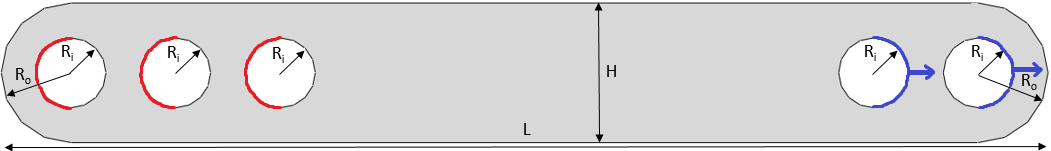
\includegraphics[width=1\textwidth]{JPfrontarticle.PNG}
    \caption{Top view of the jaw plate with five screws with dimensions and boundary conditions}
    \label{fig:BPfrontdim}
\end{figure}

\begin{table}[h]
\centering
\small
\begin{tabular}{|r|ccccc|}
\hline
\textbf{Time after im-} &  &  &  &  &  \\ 
\textbf{plantation{[}days{]}} & \textbf{0} & \textbf{28} & \textbf{77} & \textbf{124} & \textbf{170} \\ \hline
\textbf{Depth{[}mm{]}}                     & 1          & 0.95        & 0.9         & 0.85         & 0.8          \\
\textbf{H{[}mm{]}}                         & 4          & 3.95        & 3.9         & 3.85         & 3.8          \\
\textbf{R$_i$(screw){[}mm{]}}          & 1          & 1           & 1           & 1           & 1            \\
\textbf{R$_i$(no screw){[}mm{]}}       & 1          & 1.025           & 1.05           & 1.075           & 1.1            \\
\textbf{Mass loss{[}\%{]}}                 & 0          & 6.63        & 13.0        & 19.2         & 25.2         \\
\textbf{Mesh size{[}mm{]}}                 & 0.25       & 0.2375      & 0.225       & 0.2125       & 0.2          \\
\textbf{DAF{[$\mu$}m{]}}    & 10       & 9.63     & 9.25     & 8.87      & 8.48      \\ \hline
\end{tabular}
\caption{Dimensions and mesh size of the different models for the jaw plate with five screws, along with the DAF value}
\label{tab:BPdim}
\end{table}

\begin{table}[h]
\centering
\begin{tabular}{|r|l|}
\hline
\textbf{Element type}                     & Tetrahedral                     \\
\textbf{Geometric order}                  & Linear (4-node elements)        \\
\textbf{Mass scaling factor}              & 1000                            \\
\textbf{Distortion control}               & Enabled                         \\
\textbf{Distortion control: length ratio} & 0.1                             \\
\textbf{Element deletion}                 & Enabled                         \\
\textbf{Max degradation}                  & 0.95                            \\
\textbf{Processor parallellization}       & 4 processors in parallel        \\ \hline
\end{tabular}
\caption{Details about the FE analysis}
\label{tab:abaqus}
\end{table}

\subsection{Bone healing and implant load models}

According to Reina et al., the body of the mandible behaves like a long bone \cite{Reina}. Also, Korioth et al. mentioned that the jaw behaves as a beam, with the corpus (body) behaving as a hollow beam \cite{Korioth}. The 'normal' loading of the mandible occurs when eating. More specifically, the force exerted between the incisors was taken in this case study such that location of the force leads to a large moment due to the large lever arm for the moment generated in the vicinity of the fracture. Fig. \ref{fig:MandibleForceLeverArm} shows the fractured mandible with an approximate positioning of the jaw plate. The load was assumed to be vertical \cite{Reina}. The maximal biting force, recorded at the central incisors was taken as 209 N on average \cite{Mansour}. With the fracture being just posterior to the third molar, the lever arm is the distance between the central incisors and the back of the third molar, projected onto the sagittal plane. The value of 50 mm was used for this analysis, based on average values found in literature \cite{dentwiki}.

\begin{figure}[h]
    \centering
    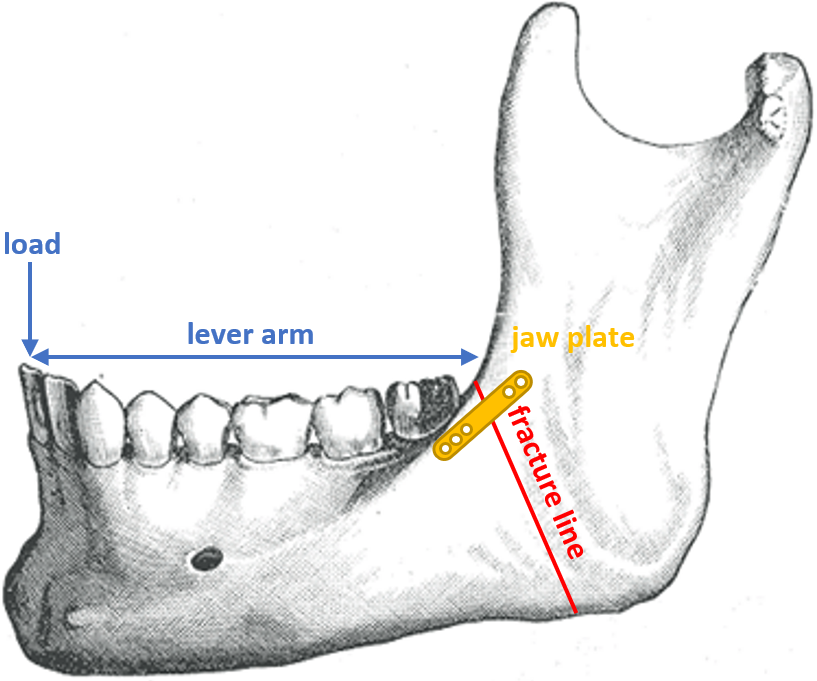
\includegraphics[width=0.7\textwidth]{MandibleForceLeverArm.PNG}
    \caption{Mandible with indication of fracture line, jaw plate, lever arm and load \cite{odora}}
    \label{fig:MandibleForceLeverArm}
\end{figure}

Fig. \ref{fig:MandibleCrossSec} shows the cross-section of the mandibular body on the left, consisting of an outer layer of cortical bone and an inner core of trabecular bone. An approximation of this cross-section using only rectangular shapes is also presented in Fig. \ref{fig:MandibleCrossSec}. This simplification was made for easier calculation of the area moment of inertia of the cross-section. The relevant dimensions for the calculation were the height and width of the outer (cortical) layer of bone as well as the thickness of this layer. These dimensions were selected based on average values for males, as they are more common to have mandible fractures \cite{Bhavik}. The average height of the mandibular body is 22.4 mm for males, as reported by Sittitavornwong et al. \cite{Sittitavornwong}. But, since the fracture line was not perpendicular to the longitudinal axis of the mandibular body, the height of the cross-section was larger than the height of the mandibular body. There was no information available on an exact fracture line, but it was estimated to be rotated 25$^{\circ}$ from the vertical. That brought the height of the mandibular body to 24.7 mm. The average width of the mandibular body is 15.9 mm, according to a study by More et al. \cite{More}. Katranji et al. found the cortical bone thickness in the mandible to be 2.06 mm on average and was assumed to be equal all around the perimeter of the cross-section \cite{Katranji}. While the jaw plate is placed a little more on the side of the mandibular body in Fig. \ref{fig:MandibleForceLeverArm}, it was placed on top of the mandibular body in the approximation in Fig. \ref{fig:MandibleCrossSec}. This was done to keep the neutral axis horizontal and to limit the complexity of the approximation. Fig. \ref{fig:MandibleJPcross} shows a close-up of the cross-section of the jaw plate with the relevant dimensions. The cross-section of the jaw plate consisted of two separate rectangles because the break in the jaw plate occurs close to a hole, which was the weakest region of the jaw plate.

\begin{figure}[h]
    \centering
    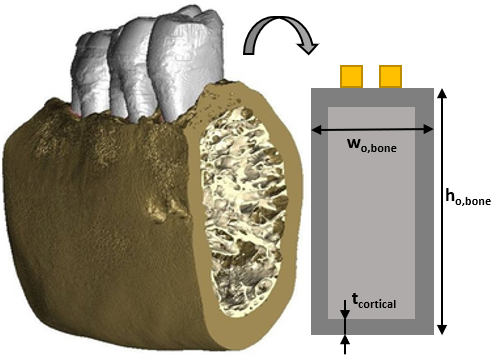
\includegraphics[width=0.7\textwidth]{MandibleCrossSec.PNG}
    \caption{cross-section of the mandibular body on the left and approximation of this cross-section with dimensions on the right \cite{plos}}
    \label{fig:MandibleCrossSec}
\end{figure}

\begin{figure}[h]
    \centering
    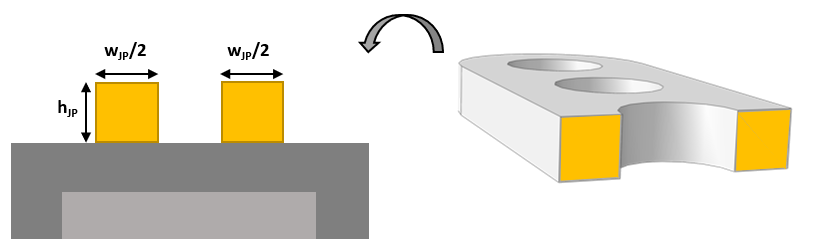
\includegraphics[width=0.9\textwidth]{MandibleJPcross.PNG}
    \caption{Close view of the cross-section of the jaw plate (indicated with JP in the figure) around the third hole (arbitrary, break does not always occur around this hole) with dimensions}
    \label{fig:MandibleJPcross}
\end{figure}

The E-modulus of the jaw plate was 44.2 GPa. The E-moduli of the cortical and trabecular bone changed over time to capture the bone healing process. To know which value of the E-modulus must be used for the cortical bone, an assumption had to be made regarding the bone healing process \cite{Voss}. Two scenarios are possible for cortical bone healing: one with direct contact between the broken bone ends and one without \cite{Marsell}. If the broken ends are pressed against each other and are rigidly fixed in place, this is called direct bone healing. The gap between the bone ends must be smaller than 0.001 mm and the interfragmentary strain must be less than 2\% for direct bone healing to occur. Cutting cones, consisting of osteoclasts, cross the fracture line and leave behind cavities, which are later filled by osteoblasts. In this way, the continuity of the bone is restored, along with the Haversian systems in the axial direction. If the gap between the bone ends is larger and relative motion is possible between the bone ends, indirect healing occurs. In this scenario, a number of different tissues are formed between the bone ends and the stability of the fracture region is gradually enhanced. In the trabecular bone, osteoblasts deposit new bone in the fracture gap by laying it on the existing bone trabeculae and along the fibers of the fibrous tissue that forms prior to bone formation \cite{Voss}.

In this case-study, the jaw plate was assumed to be able to restrict the relative movement of the bone ends of the mandible with respect to each other. For that reason, the direct bone healing scenario was more likely to occur for the cortical bone.

Lakatos et al. found the modulus of the trabecular bone in the mandible to range from 6.9 MPa to 199.5 MPa \cite{Lakatos}. The modulus of the trabecular bone after fracture started from 0 MPa and rose linearly, for the sake of simplicity, to a value of 100 MPa over the course of 168 days. The cortical bone around the fracture site was initially immature and had a modulus of around 1 GPa \cite{Isaksson}. This immature bone was replaced by stronger, mature bone with a modulus of around 6 GPa and later by compact bone \cite{hawkeye}. Because the precise rate of stiffening was not available, a rough estimation was made that made the bone modulus increase to 1.3 GPa over the same time period of 168 days.

For the implementation of the beam theory equations, the neutral axis was first calculated with a transformed-section method to take the different materials into account. Then, the area moments of inertia of the different sections were calculated. Finally, the stress in the section that corresponds to the jaw plate was calculated and was converted to a force with the use of integral expressions \cite{beamtheory}. For this, the moment in the mandibular body as a result of the biting force was used. The equations were implemented in MATLAB (Mathworks, USA) and automated to loop over different geometries of the cross-section of the plate and material properties of the bone that correspond to the degradation of the plate and the healing of the bone tissue, respectively.


\subsection{Coupling of the models}

The biodegradation simulation results were used to derive the changes in geometry on which both the FE analysis and the beam theory analysis relied. The output from the FE simulations delivered the maximum bearable force that the jaw plate can withstand while the output from the beam theory calculations delivered the actual force occurring in the jaw plate, both as a function of time. For that reason, the results could be directly compared to assess the mechanical behavior. However, the missing piece for computing the force in the jaw plate as an integral of the stress over the area of the jaw plate is the fact that stress is a linear function of $y$. That means that if the neutral axis is within the jaw plate or very close to it, the force may not be very high, while the maximal stress occurring is actually very high. If this stress is higher than ultimate tensile stress (UTS), it causes problems that might not necessarily be reflected in the total force. What this also reflects is a situation in which the loading of the jaw plate is not predominantly tensile, but instead the jaw plate is under a bending load. Using the force in the jaw plate, as computed by the integral, is only valid if the neutral axis is sufficiently far away from the jaw plate. To check this, the stress variation in the jaw plate and the location of the neutral axis were monitored.

\section{Results}
\label{sec:results}

\subsection{Biodegradation results}

The simulation of 120 days of the degradation of the jaw bone plate took 18 hours to run using 170 computing cores. Fig. \ref{fig:results_degradation} shows the visualized interface and magnesium ions release during the corrosion process. It also depicts the mass loss of the bone plate in the SBF solution over time, used to construct the mechanical analysis geometry at certain time points.

\begin{figure}[t]
\center 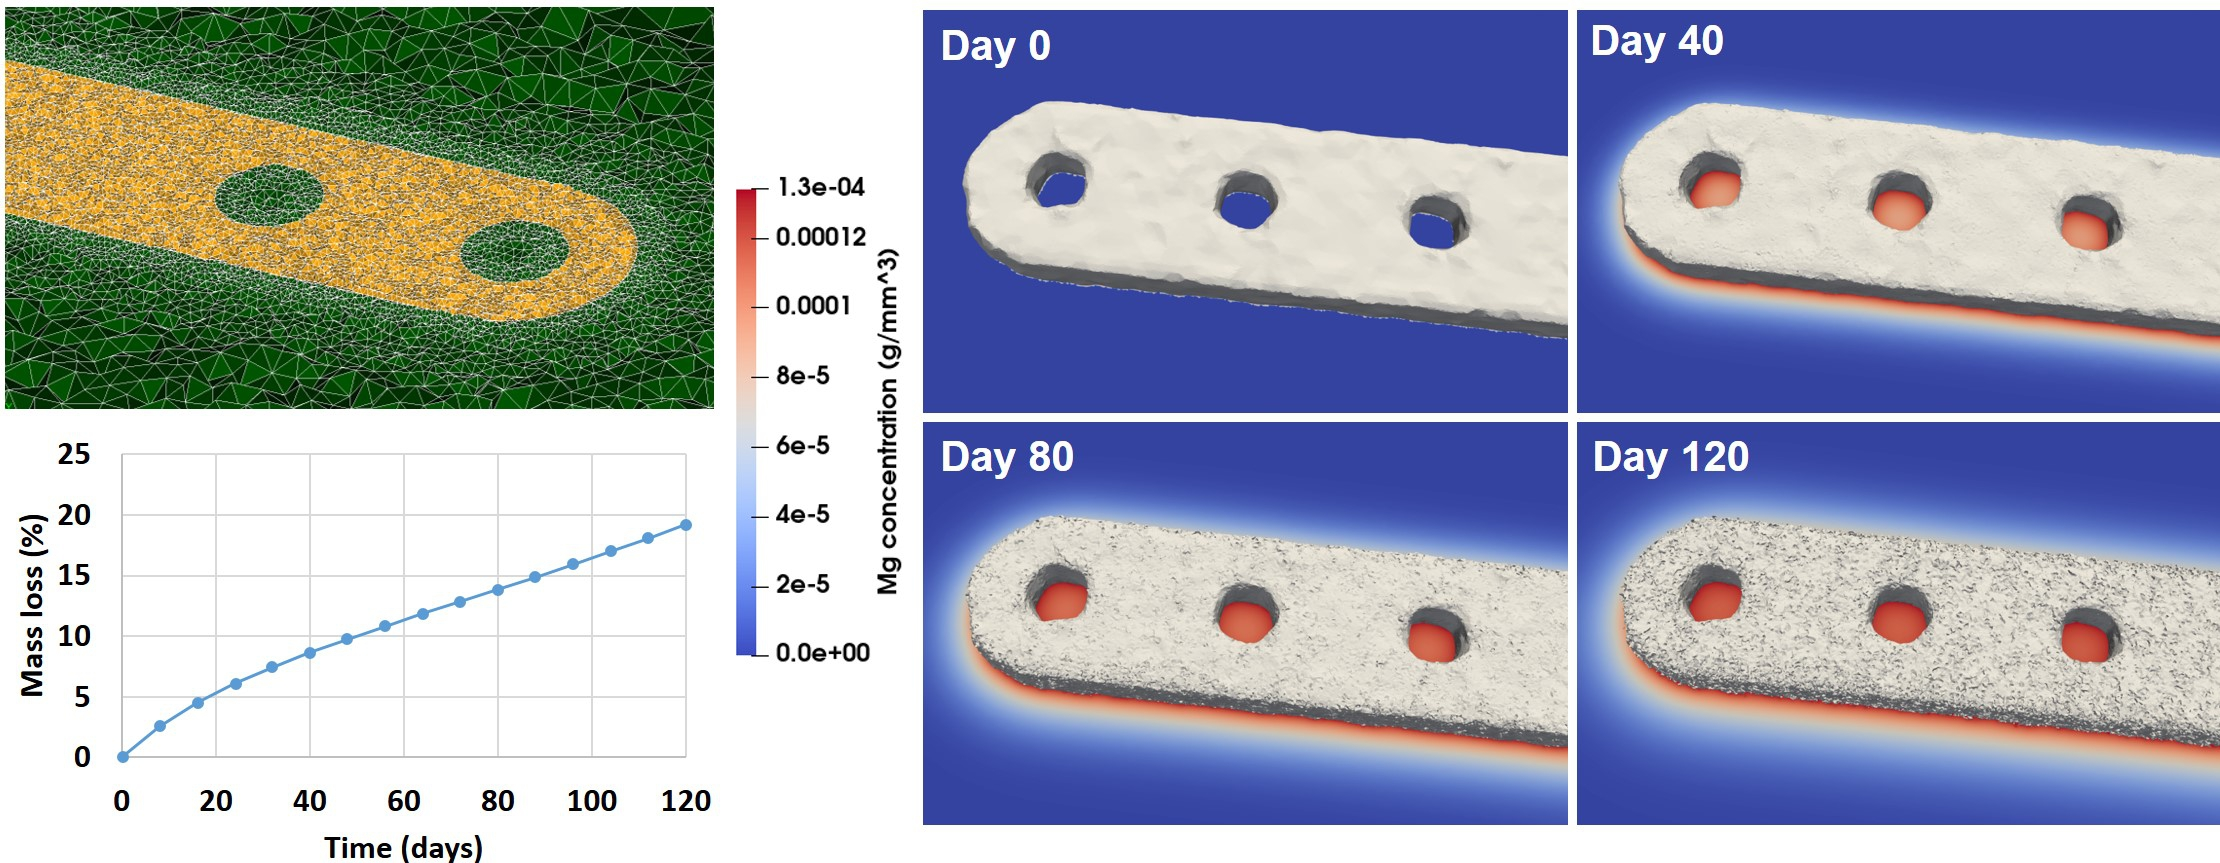
\includegraphics[width=13cm]{results_degradation.jpg}
\caption{A cross-section of the computational mesh and simulation results of the degradation model of the jaw bone plate in SBF solution as well as the mass loss graph over time. The contours display the concentration of magnesium ions on a cross-section view of the medium beside the moving surface of the bone plate at 1) 1st day (initial state), 2) 40th day, 3) 80th day, and 4) 120th day. The gray surface is the zero iso-contour of the level set function, which indicates the surface of the bone plate.} \label{fig:results_degradation}
\end{figure} 

\subsection{Sensitivity analyses}

The results from the sensitivity analyses showed that the mass scaling and the use of multiple processors for computation had no impact on the force-displacement curves. The maximum degradation only caused changes in the force-displacement curve after the maximum bearable force had been reached, and hence didn't impact the maximum bearable force. The displacement at failure and the mesh size, however, did have a strong impact on the resulting force-displacement curves. The maximum bearable force was drastically increased with an increased value of the displacement at failure. Changing the mesh size led to the opposite behavior: the maximum bearable force was lower with a larger value of the mesh size. The relationship between both was identified and the misbehavior could be eliminated by adjusting the displacement at failure to the mesh size according to the following general relationship:

\begin{equation}
X_{DAF}=0.6^{log_{0.5}(X_{mesh})} 
\end{equation}

\noindent $X_{DAF}$ is the factor with which the DAF value should be multiplied when the global mesh size is multiplied with $X_{mesh}$.

\subsubsection{Mesh check}

All models for the tensile tests had four elements in the depth. The relative difference between the maximal force for four elements in the depth compared to five elements in the depth was only 3.4\%. The computation time for four elements in the depth of this model was over 4 hours already and refining the mesh to five elements in the depth increased the computation time to over 7 hours. So, the accuracy that would be gained by refining the mesh to five elements in the depth (or further) did not justify the increase in computation time in light of this study.

\subsubsection{Neutral axis and variation in stress in the jaw plate}

The location of the neutral axis was analyzed for the five-screw case. It was assumed that in the other cases the behavior was similar. The neutral axis was closest to the jaw plate on day 0 and was at a distance of 7.6 mm from the bottom of the jaw plate at this point. That means that at this point in time, the variation in stress, which was linearly increasing from the neutral axis, was the largest (also taken into account that the force in the jaw plate was the largest at this point). So, to assess the variation of stress in the jaw plate, day 0 should be analyzed. If it is valid at that point in time, then it is valid for the remainder of the simulation. The difference in stress between the top and bottom of the jaw plate was 22.4 MPa at most, which is not too large.



\subsection{Coupled models results}

\begin{figure}[h]
    \centering
    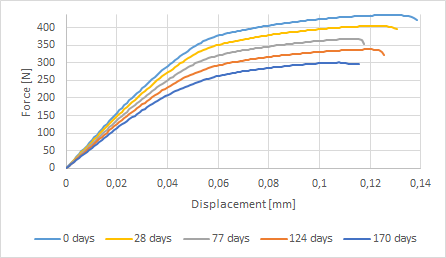
\includegraphics[width=0.8\textwidth]{BPtensgraph5screwsArticle.png}
    \caption{Results of tensile test on jaw plate with five screws with different amounts of corrosion}
    \label{fig:BPtensgraph5screws}
\end{figure}

\begin{figure}[h]
    \centering
    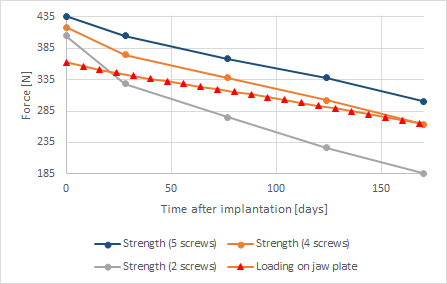
\includegraphics[width=0.8\textwidth]{BPmaxforce5screwsArticle.png}
    \caption{Maximal force that can be carried by the jaw plate in each case and estimation of load occurrence as a function of time after implantation in days for five screws}
    \label{fig:BPmaxforce5screws}
\end{figure}

The force-displacement curves for the case with five screws are shown in Fig. \ref{fig:BPtensgraph5screws}, the cases with four and two screws gave similar force-displacement curves. The strength of the jaw plates was characterized by the maximal values from the force-displacement curves. In Fig. \ref{fig:BPmaxforce5screws}, the strength-curves of the jaw plate for the three cases are shown and compared to the loading on the jaw plate, as calculated with beam theory. Comparing the three strength-curves, it could be concluded that leaving more holes open led to a weaker part initially and a faster deterioration of the strength with time as a result of corrosion. In the five-screw case, the strength remained higher than the loading for the simulated time period and hence no failure occurred. In the four- and two-screw cases, failure did occur after about 170 and 20 days respectively.


\section{Discussion}

In this work, a coupled mechanical-degradation model was presented to study the effect of biodegradation on the mechanical stability of implants for biodegradable mandibular plates. Three different cases were considered, in each of which a different number of implant holes were left unscrewed. One aspect of the difference between the three cases is the surface that was exposed to body fluids. The extra surfaces exposed to body fluids in the four- and two-screw cases were inside the open holes, which were critical regions. The "extra" corrosion inside the holes had an impact on the strength, as the results of Fig. \ref{fig:BPmaxforce5screws} show. The other aspect of the difference between the cases has is on the boundary conditions that represented the screws pulling on the jaw plate. The differences in the maximal force on day 0 between the three cases is a result of the boundary conditions only since there was no corrosion at this point in time and the models were identical. 

The use of a "universal" jaw plate with multiple holes allows the jaw plate to be used in various situations involving mandible fractures. Depending on the exact location of fracture lines and the presence of stronger and weaker sections of bone, the amount and placement of screws can be decided upon. The downside to this is that the differences in mechanical behavior and the change thereof as a result of corrosion between the different cases (5/4/2 screws) can lead to unexpected results if not anticipated correctly by the jaw plate designer/surgeon. A patient-specific jaw plate can be designed to meet a specific mechanical behavior. The placement of holes and the presence or absence of screws can then be a powerful tool for obtaining the desired mechanical behavior of the jaw plate.

The results of the strength simulations provided useful knowledge about the limits in terms of the mechanical strength of the jaw plate and how that evolved during the biodegradation process. Matched with an accurate characterization of the loading, the point at which the jaw plate fails could be predicted. The loading on the jaw plate was derived from the maximal biting force. This has to be taken into account when interpreting the results. The jaw plate would fail if the maximal biting force would be exerted after the point at which the strength curve falls below the loading curve. In practice, the strength of the jaw plate and the way in which this evolves during the biodegradation process are influenced by a range of parameters. Most of these are fixed by the situation/patient: mandible dimensions, bone properties, fracture line geometry, etc. Others are, however, free to be chosen by the implant designer: the jaw plate material and geometry, the location, the number of screws, etc. Certain restrictions on what food may be eaten by the patient for a certain time period can be given to reduce the maximal biting force. 

The design of this jaw plate is a complex task that can be modified in various ways. Fig. \ref{fig:FlowChartJP} gives an overview of an automated workflow that incorporates the concepts from this study into the iterative design of the jaw plate. With the use of initial data of the mandible and the jaw plate, the mechanical behavior can be determined. Likely, the behavior of the initial design is not as desired. For that reason, the design process is based on the iterative adjustment of the parameters to ultimately obtain the desired mechanical behavior. The material of the jaw plate can be chosen to be stronger or weaker, impacting the estimation of the loading on the jaw plate and the simulation of the strength of the jaw plate. The degradation-related properties of the material impact the corrosion simulation, which in turn determines the geometry changes for the simulation of strength. The geometry of the jaw plate can have similar effects as the material, impacting both strength and degradation behavior. For example, the rate of degradation can be modulated by increasing or decreasing the surface-area-to-volume ratio of the jaw plate. A high surface-area-to-volume ratio (imagine a wide but very thin jaw plate) leads to a faster loss of material (and strength) since the area exposed to body fluids is high. The opposite is true for a low surface-area-to-volume ratio (imagine a jaw plate with a square cross-section perpendicular to the longitudinal axis). The location changes the type of loading on the jaw plate, and it is important that this loading situation is reflected in the simulation of the strength. For example, it is not useful to submit the jaw plate models to a tensile test if the jaw plate is actually experiencing a bending moment once implanted. %In the flowchart, the green box indicates the scope of the Master's Thesis on which this article is based.

\begin{figure}[h]
    \centering
    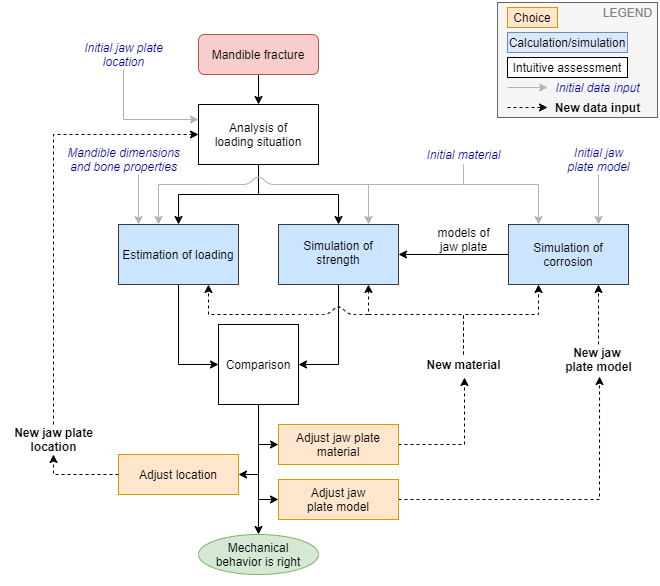
\includegraphics[width=1\textwidth]{FlowChartJP.png}
    \caption{Flow chart for the process of iteratively designing a suitable jaw plate}
    \label{fig:FlowChartJP}
\end{figure}

\section{Future perspectives}
\label{sec:future}

The validity and accuracy of the curves depend on the data that is used to create them and on the degree to which the simplifications deviate from reality. The E-moduli of the bone could be obtained from dedicated experiments and plugged into the beam theory equations to more accurately define the load on the jaw plate. Alternatively, an FE model of the entire mandible with jaw plate could replace the combination of the beam theory and the FE analysis of the jaw plate separately. This would be more accurate since the loading is not approximated. Another interesting thing to take into account could be the amount of displacement before failure. The area under the force-displacement curve is an indication of energy absorption. The addition of localized corrosion to the simulations could also be interesting, since the reality of corrosion always involves a combination of localized and uniform corrosion. While the relative change in force values led to interesting conclusions, the absolute values of the results obtained in this study were not validated. Manufacturing real samples, immersing them in SBF, and objecting them to a tensile test would give \textit{in vitro}results that can be compared to the simulation predictions.  


\section*{Acknowledgments}

This research is financially supported by the Prosperos project, funded by the Interreg VA Flanders – The Netherlands program, CCI grant no. 2014TC16RFCB046 and by the Fund for Scientific Research Flanders (FWO), grant G085018N . LG acknowledges support from the European Research Council under the European Union’s Horizon 2020 research and innovation programme, ERC CoG 772418. The computational resources and services used in this work were provided by the VSC (Flemish Supercomputer Center), funded by the Research Foundation - Flanders (FWO) and the Flemish Government – department EWI.


%%%%%%%%%%%%%%%%%%%%%%%%%%%%%%%%%%%%%%%%%%%%%%%%%%
% Keep the following \cleardoublepage at the end of this file, 
% otherwise \includeonly includes empty pages.
\cleardoublepage

